\chapter{Risk as Controllable Variables}

This chapter is based on a short School of Hard Knocks entrepreneurship interview, curated by LazyingArt LLC with Video2Book. The exchange asks a practical question: what is the most important part of taking risks in order to become successful, and what risks outside finance may be required along the way? The answer does not praise risk for its own sake. It turns risk into a sorting procedure: first identify what can be mitigated, fixed, or controlled; only then ask whether the remaining uncertainty fits the entrepreneur's tolerance.

\section{The Question: What Makes Risk Worth Taking?}

The question arrives in two parts. First, what matters most about taking risks to become successful? Second, are there non-financial risks one has to take to get where one is going? That second part matters. The answer is not only about capital. It is about judgment, control, and the willingness to live with what remains uncertain.

The speaker begins by widening the field: there are many ways to think about risk. Then he narrows it quickly. In the companies he works with now, and in places where he has worked before, the useful question is not simply whether a situation is risky. It is whether the risk can be mitigated or fixed.

\begin{definition}
A \emph{risk variable} is a material uncertainty that can affect the outcome of a decision. A variable is \emph{controllable} if the entrepreneur can meaningfully influence, mitigate, or repair it. A variable is \emph{uncontrollable} if it lies outside the entrepreneur's practical reach.
\end{definition}

We will use a little notation, but only as bookkeeping for the examples in the interview:
\begin{align}
n&=\text{number of material risk variables},\\
c&=\text{number we can control, mitigate, or fix},\\
u&=n-c=\text{number left outside our control}.
\end{align}
The corresponding controllability ratio is
\begin{equation}
\rho=\frac{c}{n}.
\end{equation}
This ratio is not a probability of success. It is a compact way of expressing the distinction the speaker is making: some risks can be worked on, while others can only be endured.

\section{Risk as Control, Not Drama}

A tempting but weak theory of entrepreneurship says that risk is valuable because it is bold. The speaker rejects that romance. If a risk is way outside one's control, then it remains outside one's control. The plainness of the statement is the point.

The test is operational. Can we act on the moving parts? Can we reduce the danger? Can we repair the failure mode if it appears? A risk that can be mitigated belongs to the domain of management and execution. A risk with too many uncontrolled variables is closer to a flyer.

\subsection{Question \& Answer}

\paragraph{Question.}
When is a risk worth taking?

\paragraph{Answer.}
A risk is worth considering when enough of the important variables are controllable, mitigable, or fixable. If most of the important variables are outside control, the decision is not disciplined risk; it is a flyer. Even when the structure looks favorable, the decision still depends on personal risk tolerance.

A cautious mnemonic is
\begin{equation}
\text{disciplined risk}
\quad \approx \quad
\text{controllability}
+
\text{tolerance for the unresolved part}.
\end{equation}
The symbol \(\approx\) is deliberate. The interview gives a practical test, not a universal law.

\section{Counting the Variables}

The speaker makes the test concrete with numbers. Suppose there are six risky variables and only two can be controlled. In our notation,
\begin{align}
n&=6, & c&=2, & u&=4,\\
\rho&=\frac{2}{6}=\frac{1}{3}.
\end{align}
The speaker's judgment is that this is not a good idea. We should not take a flyer while admitting that most of the important variables are loose.

Now change the structure. Suppose there are three risky variables and two can be controlled:
\begin{align}
n&=3, & c&=2, & u&=1,\\
\rho&=\frac{2}{3}.
\end{align}
The same number of controlled variables now sits in a different world. Two controlled variables out of six leaves four outside control. Two controlled variables out of three leaves only one. That is why the second case has, in the speaker's phrase, a pretty good shot.

\subsection{Worked Example: Same Control, Different Denominator}

The mistake would be to look only at \(c=2\). In both examples we control two variables. The useful comparison is the fraction of the decision that can be acted on:
\begin{align}
\rho_{\mathrm{loose}} &= \frac{2}{6}=\frac{1}{3},\\
\rho_{\mathrm{tighter}} &= \frac{2}{3}.
\end{align}
Therefore
\begin{equation}
\rho_{\mathrm{tighter}}>\rho_{\mathrm{loose}}.
\end{equation}
This inequality is the mathematical core of the interview's example. It does not say that the second decision will succeed. It says that the second decision gives the entrepreneur more of the relevant surface area to work on.

\begin{table}
\centering
\begin{tabular}{p{0.25\linewidth} p{0.24\linewidth} p{0.38\linewidth}}
Risk situation & Control position & Implied judgment \\
Six risky variables & Control two & Too many loose variables; avoid the flyer \\
Three risky variables & Control two & Better shot; enough may be controllable to proceed \\
\end{tabular}
\caption{Transcript-derived reconstruction of the speaker's variable-counting heuristic.}
\end{table}

The table should not be read as a threshold rule. The interview does not define a cutoff such as \(\rho>1/2\). It gives a disciplined way to compare situations before emotion takes over.

\section{A Decision Diagram for Mitigable Risk}

Since the interview supplies no board drawing to preserve, the diagram below is a clean reconstruction of the spoken logic. It is intentionally vertical and narrow: the chapter needs a portable decision flow, not a sprawling model of risk.

\begin{figure}
\centering
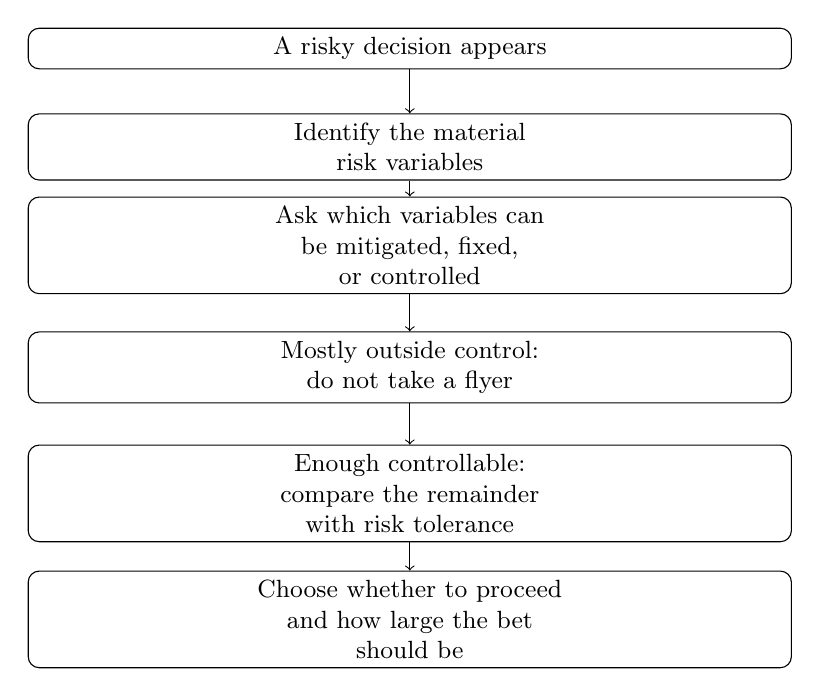
\begin{tikzpicture}[x=1cm,y=1cm,every node/.style={font=\small}]
\node[draw,rounded corners,align=center,text width=.78\linewidth] (a) at (0,0) {A risky decision appears};
\node[draw,rounded corners,align=center,text width=.78\linewidth] (b) at (0,-1.25) {Identify the material\\ risk variables};
\node[draw,rounded corners,align=center,text width=.78\linewidth] (c) at (0,-2.50) {Ask which variables can\\ be mitigated, fixed,\\ or controlled};
\node[draw,rounded corners,align=center,text width=.78\linewidth] (d) at (0,-4.05) {Mostly outside control:\\ do not take a flyer};
\node[draw,rounded corners,align=center,text width=.78\linewidth] (e) at (0,-5.65) {Enough controllable:\\ compare the remainder\\ with risk tolerance};
\node[draw,rounded corners,align=center,text width=.78\linewidth] (f) at (0,-7.25) {Choose whether to proceed\\ and how large the bet\\ should be};
\draw[->] (a) -- (b);
\draw[->] (b) -- (c);
\draw[->] (c) -- (d);
\draw[->] (d) -- (e);
\draw[->] (e) -- (f);
\end{tikzpicture}
\caption{A pocket-size reconstruction of the transcript's risk-control sequence.}
\end{figure}

The diagram is sequential because that is how the answer unfolds. First we name the variables. Then we ask which ones can be acted on. Only after that do we bring in personal tolerance and bet size.

\section{Risk Tolerance and Bet Size}

After the variable-counting example, the speaker pivots to risk tolerance. This is not an afterthought. It prevents the notation from becoming mechanical. Two people can face the same \(n\), \(c\), and \(\rho\), yet make different decisions because they cannot carry the same unresolved uncertainty.

Let \(T\) denote a person's tolerance for the remaining risk. We should not pretend that \(T\) is measured precisely here. It is a name for a constraint:
\begin{equation}
\text{decision judgment depends on }(\rho,T),
\end{equation}
where \(\rho\) describes the structure of the situation and \(T\) describes the person's willingness to carry what cannot be controlled.

The next question is not only whether to act, but how much to commit. If \(B\) denotes the size of the bet, the interview's final example rests on a qualitative ordering:
\begin{equation}
B_{\mathrm{small}}<B_{\mathrm{large}}.
\end{equation}
A larger commitment creates larger exposure. It also creates the possibility of capturing more of the upside if the decision works.

\section{The Musk Example: Concentrated Upside}

The closing anecdote is Elon Musk after PayPal. The speaker says Musk took basically all he made at PayPal, put it into another deal, and that deal hit huge. The example is not offered as a rule that every entrepreneur should imitate. It is evidence of unusually high risk tolerance joined to a concentrated bet.

\paragraph{Anecdote.}
The PayPal proceeds become the stake. Tesla becomes the next opportunity. The commitment is large rather than symbolic.

\paragraph{Claim.}
The speaker says that if Musk had put only a little bit in, he would not be worth \(\$250\) billion. That figure should be preserved as a spoken interview claim.

\paragraph{Mechanism.}
The mechanism is not mysterious: smaller exposure limits downside, but it also limits participation in upside. In qualitative form,
\begin{equation}
\text{larger concentrated bet}
\quad \Longrightarrow \quad
\text{larger possible upside and larger exposure}.
\end{equation}
The anecdote completes the arc of the answer. We began with the broad question of risk and success. We then sorted risk by controllability. Finally, we saw that tolerance determines not only whether one proceeds, but also the size of the commitment.

\section{Summary}

The chapter's practical lesson is narrow and strong. Do not begin by asking whether a risk is heroic. Begin by asking what variables matter and which of them can be mitigated, fixed, or controlled. If too many variables are outside control, the decision is a flyer. If enough variables can be acted on, the risk becomes a candidate for entrepreneurial judgment.

The two numerical examples preserve the core comparison:
\begin{equation}
\frac{2}{6}
\quad \text{is a weaker control position than} \quad
\frac{2}{3}.
\end{equation}
But the ratio is not the whole story. A disciplined entrepreneur also asks whether the remaining uncertainty fits personal risk tolerance, and whether the size of the bet matches the upside being pursued.